
%% bare_conf.tex
%% V1.3
%% 2007/01/11
%% by Michael Shell
%% See:
%% http://www.michaelshell.org/
%% for current contact information.
%%
%% This is a skeleton file demonstrating the use of IEEEtran.cls
%% (requires IEEEtran.cls version 1.7 or later) with an IEEE conference paper.
%%
%% Support sites:
%% http://www.michaelshell.org/tex/ieeetran/
%% http://www.ctan.org/tex-archive/macros/latex/contrib/IEEEtran/
%% and
%% http://www.ieee.org/

%%*************************************************************************
%% Legal Notice:
%% This code is offered as-is without any warranty either expressed or
%% implied; without even the implied warranty of MERCHANTABILITY or
%% FITNESS FOR A PARTICULAR PURPOSE! 
%% User assumes all risk.
%% In no event shall IEEE or any contributor to this code be liable for
%% any damages or losses, including, but not limited to, incidental,
%% consequential, or any other damages, resulting from the use or misuse
%% of any information contained here.
%%
%% All comments are the opinions of their respective authors and are not
%% necessarily endorsed by the IEEE.
%%
%% This work is distributed under the LaTeX Project Public License (LPPL)
%% ( http://www.latex-project.org/ ) version 1.3, and may be freely used,
%% distributed and modified. A copy of the LPPL, version 1.3, is included
%% in the base LaTeX documentation of all distributions of LaTeX released
%% 2003/12/01 or later.
%% Retain all contribution notices and credits.
%% ** Modified files should be clearly indicated as such, including  **
%% ** renaming them and changing author support contact information. **
%%
%% File list of work: IEEEtran.cls, IEEEtran_HOWTO.pdf, bare_adv.tex,
%%                    bare_conf.tex, bare_jrnl.tex, bare_jrnl_compsoc.tex
%%*************************************************************************

% *** Authors should verify (and, if needed, correct) their LaTeX system  ***
% *** with the testflow diagnostic prior to trusting their LaTeX platform ***
% *** with production work. IEEE's font choices can trigger bugs that do  ***
% *** not appear when using other class files.                            ***
% The testflow support page is at:
% http://www.michaelshell.org/tex/testflow/



% Note that the a4paper option is mainly intended so that authors in
% countries using A4 can easily print to A4 and see how their papers will
% look in print - the typesetting of the document will not typically be
% affected with changes in paper size (but the bottom and side margins will).
% Use the testflow package mentioned above to verify correct handling of
% both paper sizes by the user's LaTeX system.
%
% Also note that the "draftcls" or "draftclsnofoot", not "draft", option
% should be used if it is desired that the figures are to be displayed in
% draft mode.
%
\documentclass[10pt, conference, compsocconf]{IEEEtran}
% Add the compsocconf option for Computer Society conferences.
%
% If IEEEtran.cls has not been installed into the LaTeX system files,
% manually specify the path to it like:
% \documentclass[conference]{../sty/IEEEtran}





% Some very useful LaTeX packages include:
% (uncomment the ones you want to load)


% *** MISC UTILITY PACKAGES ***
%
%\usepackage{ifpdf}
% Heiko Oberdiek's ifpdf.sty is very useful if you need conditional
% compilation based on whether the output is pdf or dvi.
% usage:
% \ifpdf
%   % pdf code
% \else
%   % dvi code
% \fi
% The latest version of ifpdf.sty can be obtained from:
% http://www.ctan.org/tex-archive/macros/latex/contrib/oberdiek/
% Also, note that IEEEtran.cls V1.7 and later provides a builtin
% \ifCLASSINFOpdf conditional that works the same way.
% When switching from latex to pdflatex and vice-versa, the compiler may
% have to be run twice to clear warning/error messages.

\usepackage{tabularx}
\usepackage{booktabs}






% *** CITATION PACKAGES ***
%
\usepackage{cite}
% cite.sty was written by Donald Arseneau
% V1.6 and later of IEEEtran pre-defines the format of the cite.sty package
% \cite{} output to follow that of IEEE. Loading the cite package will
% result in citation numbers being automatically sorted and properly
% "compressed/ranged". e.g., [1], [9], [2], [7], [5], [6] without using
% cite.sty will become [1], [2], [5]--[7], [9] using cite.sty. cite.sty's
% \cite will automatically add leading space, if needed. Use cite.sty's
% noadjust option (cite.sty V3.8 and later) if you want to turn this off.
% cite.sty is already installed on most LaTeX systems. Be sure and use
% version 4.0 (2003-05-27) and later if using hyperref.sty. cite.sty does
% not currently provide for hyperlinked citations.
% The latest version can be obtained at:
% http://www.ctan.org/tex-archive/macros/latex/contrib/cite/
% The documentation is contained in the cite.sty file itself.






% *** GRAPHICS RELATED PACKAGES ***
%
\usepackage{graphicx}
\ifCLASSINFOpdf
  %\usepackage[pdftex]{graphicx}
  % declare the path(s) where your graphic files are
  % \graphicspath{{../pdf/}{../jpeg/}}
  % and their extensions so you won't have to specify these with
  % every instance of \includegraphics
  %\DeclareGraphicsExtensions{.pdf,.jpeg,.png}
\else
  % or other class option (dvipsone, dvipdf, if not using dvips). graphicx
  % will default to the driver specified in the system graphics.cfg if no
  % driver is specified.
  % \usepackage[dvips]{graphicx}
  % declare the path(s) where your graphic files are
  % \graphicspath{{../eps/}}
  % and their extensions so you won't have to specify these with
  % every instance of \includegraphics
  % \DeclareGraphicsExtensions{.eps}
\fi
% graphicx was written by David Carlisle and Sebastian Rahtz. It is
% required if you want graphics, photos, etc. graphicx.sty is already
% installed on most LaTeX systems. The latest version and documentation can
% be obtained at: 
% http://www.ctan.org/tex-archive/macros/latex/required/graphics/
% Another good source of documentation is "Using Imported Graphics in
% LaTeX2e" by Keith Reckdahl which can be found as epslatex.ps or
% epslatex.pdf at: http://www.ctan.org/tex-archive/info/
%
% latex, and pdflatex in dvi mode, support graphics in encapsulated
% postscript (.eps) format. pdflatex in pdf mode supports graphics
% in .pdf, .jpeg, .png and .mps (metapost) formats. Users should ensure
% that all non-photo figures use a vector format (.eps, .pdf, .mps) and
% not a bitmapped formats (.jpeg, .png). IEEE frowns on bitmapped formats
% which can result in "jaggedy"/blurry rendering of lines and letters as
% well as large increases in file sizes.
%
% You can find documentation about the pdfTeX application at:
% http://www.tug.org/applications/pdftex





% *** MATH PACKAGES ***
%
%\usepackage[cmex10]{amsmath}
% A popular package from the American Mathematical Society that provides
% many useful and powerful commands for dealing with mathematics. If using
% it, be sure to load this package with the cmex10 option to ensure that
% only type 1 fonts will utilized at all point sizes. Without this option,
% it is possible that some math symbols, particularly those within
% footnotes, will be rendered in bitmap form which will result in a
% document that can not be IEEE Xplore compliant!
%
% Also, note that the amsmath package sets \interdisplaylinepenalty to 10000
% thus preventing page breaks from occurring within multiline equations. Use:
%\interdisplaylinepenalty=2500
% after loading amsmath to restore such page breaks as IEEEtran.cls normally
% does. amsmath.sty is already installed on most LaTeX systems. The latest
% version and documentation can be obtained at:
% http://www.ctan.org/tex-archive/macros/latex/required/amslatex/math/





% *** SPECIALIZED LIST PACKAGES ***
%
%\usepackage{algorithmic}
% algorithmic.sty was written by Peter Williams and Rogerio Brito.
% This package provides an algorithmic environment fo describing algorithms.
% You can use the algorithmic environment in-text or within a figure
% environment to provide for a floating algorithm. Do NOT use the algorithm
% floating environment provided by algorithm.sty (by the same authors) or
% algorithm2e.sty (by Christophe Fiorio) as IEEE does not use dedicated
% algorithm float types and packages that provide these will not provide
% correct IEEE style captions. The latest version and documentation of
% algorithmic.sty can be obtained at:
% http://www.ctan.org/tex-archive/macros/latex/contrib/algorithms/
% There is also a support site at:
% http://algorithms.berlios.de/index.html
% Also of interest may be the (relatively newer and more customizable)
% algorithmicx.sty package by Szasz Janos:
% http://www.ctan.org/tex-archive/macros/latex/contrib/algorithmicx/




% *** ALIGNMENT PACKAGES ***
%
%\usepackage{array}
% Frank Mittelbach's and David Carlisle's array.sty patches and improves
% the standard LaTeX2e array and tabular environments to provide better
% appearance and additional user controls. As the default LaTeX2e table
% generation code is lacking to the point of almost being broken with
% respect to the quality of the end results, all users are strongly
% advised to use an enhanced (at the very least that provided by array.sty)
% set of table tools. array.sty is already installed on most systems. The
% latest version and documentation can be obtained at:
% http://www.ctan.org/tex-archive/macros/latex/required/tools/


%\usepackage{mdwmath}
%\usepackage{mdwtab}
% Also highly recommended is Mark Wooding's extremely powerful MDW tools,
% especially mdwmath.sty and mdwtab.sty which are used to format equations
% and tables, respectively. The MDWtools set is already installed on most
% LaTeX systems. The lastest version and documentation is available at:
% http://www.ctan.org/tex-archive/macros/latex/contrib/mdwtools/


% IEEEtran contains the IEEEeqnarray family of commands that can be used to
% generate multiline equations as well as matrices, tables, etc., of high
% quality.


%\usepackage{eqparbox}
% Also of notable interest is Scott Pakin's eqparbox package for creating
% (automatically sized) equal width boxes - aka "natural width parboxes".
% Available at:
% http://www.ctan.org/tex-archive/macros/latex/contrib/eqparbox/





% *** SUBFIGURE PACKAGES ***
%\usepackage[tight,footnotesize]{subfigure}
% subfigure.sty was written by Steven Douglas Cochran. This package makes it
% easy to put subfigures in your figures. e.g., "Figure 1a and 1b". For IEEE
% work, it is a good idea to load it with the tight package option to reduce
% the amount of white space around the subfigures. subfigure.sty is already
% installed on most LaTeX systems. The latest version and documentation can
% be obtained at:
% http://www.ctan.org/tex-archive/obsolete/macros/latex/contrib/subfigure/
% subfigure.sty has been superceeded by subfig.sty.



%\usepackage[caption=false]{caption}
%\usepackage[font=footnotesize]{subfig}
% subfig.sty, also written by Steven Douglas Cochran, is the modern
% replacement for subfigure.sty. However, subfig.sty requires and
% automatically loads Axel Sommerfeldt's caption.sty which will override
% IEEEtran.cls handling of captions and this will result in nonIEEE style
% figure/table captions. To prevent this problem, be sure and preload
% caption.sty with its "caption=false" package option. This is will preserve
% IEEEtran.cls handing of captions. Version 1.3 (2005/06/28) and later 
% (recommended due to many improvements over 1.2) of subfig.sty supports
% the caption=false option directly:
%\usepackage[caption=false,font=footnotesize]{subfig}
%
% The latest version and documentation can be obtained at:
% http://www.ctan.org/tex-archive/macros/latex/contrib/subfig/
% The latest version and documentation of caption.sty can be obtained at:
% http://www.ctan.org/tex-archive/macros/latex/contrib/caption/




% *** FLOAT PACKAGES ***
%
%\usepackage{fixltx2e}
% fixltx2e, the successor to the earlier fix2col.sty, was written by
% Frank Mittelbach and David Carlisle. This package corrects a few problems
% in the LaTeX2e kernel, the most notable of which is that in current
% LaTeX2e releases, the ordering of single and double column floats is not
% guaranteed to be preserved. Thus, an unpatched LaTeX2e can allow a
% single column figure to be placed prior to an earlier double column
% figure. The latest version and documentation can be found at:
% http://www.ctan.org/tex-archive/macros/latex/base/



%\usepackage{stfloats}
% stfloats.sty was written by Sigitas Tolusis. This package gives LaTeX2e
% the ability to do double column floats at the bottom of the page as well
% as the top. (e.g., "\begin{figure*}[!b]" is not normally possible in
% LaTeX2e). It also provides a command:
%\fnbelowfloat
% to enable the placement of footnotes below bottom floats (the standard
% LaTeX2e kernel puts them above bottom floats). This is an invasive package
% which rewrites many portions of the LaTeX2e float routines. It may not work
% with other packages that modify the LaTeX2e float routines. The latest
% version and documentation can be obtained at:
% http://www.ctan.org/tex-archive/macros/latex/contrib/sttools/
% Documentation is contained in the stfloats.sty comments as well as in the
% presfull.pdf file. Do not use the stfloats baselinefloat ability as IEEE
% does not allow \baselineskip to stretch. Authors submitting work to the
% IEEE should note that IEEE rarely uses double column equations and
% that authors should try to avoid such use. Do not be tempted to use the
% cuted.sty or midfloat.sty packages (also by Sigitas Tolusis) as IEEE does
% not format its papers in such ways.





% *** PDF, URL AND HYPERLINK PACKAGES ***
%
%\usepackage{url}
% url.sty was written by Donald Arseneau. It provides better support for
% handling and breaking URLs. url.sty is already installed on most LaTeX
% systems. The latest version can be obtained at:
% http://www.ctan.org/tex-archive/macros/latex/contrib/misc/
% Read the url.sty source comments for usage information. Basically,
% \url{my_url_here}.





% *** Do not adjust lengths that control margins, column widths, etc. ***
% *** Do not use packages that alter fonts (such as pslatex).         ***
% There should be no need to do such things with IEEEtran.cls V1.6 and later.
% (Unless specifically asked to do so by the journal or conference you plan
% to submit to, of course. )


% correct bad hyphenation here
\hyphenation{op-tical net-works semi-conduc-tor}


\begin{document}
%
% paper title
% can use linebreaks \\ within to get better formatting as desired
\title{Author Identification on Twitter (Milestone Report)}


% author names and affiliations
% use a multiple column layout for up to two different
% affiliations

\author{\IEEEauthorblockN{Antonio Castro}
\IEEEauthorblockA{antonio.alfredo.castro@gmail.com}\\
\and
\IEEEauthorblockN{Brian Lindauer}
\IEEEauthorblockA{brian@shendauer.com}
}

% conference papers do not typically use \thanks and this command
% is locked out in conference mode. If really needed, such as for
% the acknowledgment of grants, issue a \IEEEoverridecommandlockouts
% after \documentclass

% for over three affiliations, or if they all won't fit within the width
% of the page, use this alternative format:
% 
%\author{\IEEEauthorblockN{Michael Shell\IEEEauthorrefmark{1},
%Homer Simpson\IEEEauthorrefmark{2},
%James Kirk\IEEEauthorrefmark{3}, 
%Montgomery Scott\IEEEauthorrefmark{3} and
%Eldon Tyrell\IEEEauthorrefmark{4}}
%\IEEEauthorblockA{\IEEEauthorrefmark{1}School of Electrical and Computer Engineering\\
%Georgia Institute of Technology,
%Atlanta, Georgia 30332--0250\\ Email: see http://www.michaelshell.org/contact.html}
%\IEEEauthorblockA{\IEEEauthorrefmark{2}Twentieth Century Fox, Springfield, USA\\
%Email: homer@thesimpsons.com}
%\IEEEauthorblockA{\IEEEauthorrefmark{3}Starfleet Academy, San Francisco, California 96678-2391\\
%Telephone: (800) 555--1212, Fax: (888) 555--1212}
%\IEEEauthorblockA{\IEEEauthorrefmark{4}Tyrell Inc., 123 Replicant Street, Los Angeles, California 90210--4321}}




% use for special paper notices
%\IEEEspecialpapernotice{(Invited Paper)}




% make the title area
\maketitle


% \begin{abstract}
% The abstract goes here. DO NOT USE SPECIAL CHARACTERS, SYMBOLS, OR MATH IN YOUR TITLE OR ABSTRACT.

% \end{abstract}

% \begin{IEEEkeywords}
% component; formatting; style; styling;

% \end{IEEEkeywords}


% For peer review papers, you can put extra information on the cover
% page as needed:
% \ifCLASSOPTIONpeerreview
% \begin{center} \bfseries EDICS Category: 3-BBND \end{center}
% \fi
%
% For peerreview papers, this IEEEtran command inserts a page break and
% creates the second title. It will be ignored for other modes.
\IEEEpeerreviewmaketitle



\section{Introduction}
% no \IEEEPARstart
As of June 2012, Twitter has 500M users, 140M of whom are in the
United States. These users, especially those outside of the United
States, may assume that they have a certain level of anonymity among
this sea of tweets. Our project investigates whether the identity of
an anonymous Twitter user can, in fact, be uncovered using only
linguistic stylometry. Authorship recognition is a very well-studied
domain, but the scale is almost always limited to no more than a few
hundred authors. Narayanan, et al.\cite{Narayanan} study authorship recognition at
Internet scale, by looking at the characteristics of different
classifiers when applied to a corpus of approximately 100k
blogs. Starting with the set of features, classifiers, and
normalization methods that yielded the best results over blog data in
that paper we adapt them to Twitter data and measure the results.
% You must have at least 2 lines in the paragraph with the drop letter
% (should never be an issue)

\section{Data Collection}
Our goal was to obtain a training set across at least 1000 users and
have at least 1000 tweets per user to enable our feature set to have
enough data due to the sparsity of our planned data features. Our
first data collection task was to identify an appropriate subset of
the Twitter users and Twitter users in which we have prior knowledge
that they are authored by the same user.

Table I describes the various sources we attempted gathering and how we ended up using the data.
\begin{table}[!h]
  \centering
  \begin{tabularx}{\linewidth}{X X X}
    \toprule
    \bf{Source} & \bf{Desired Usage} & \bf{Actual Usage} \\ \midrule
    Klout & We attempted to gather the top thousand klout users as a method of gathering users with rich content. & Not used. Only small lists of top klout rankings are published and we were not able to obtain a list longer than 10-20. \\ \midrule
    Twitter Firehose & Obtain tons of tweets across a massive number of users. & Not used. While the data was broad, it did not provide us with a long enough history of any individual user to populate our sparse set of features. \\ \midrule
    Twitaholic & Provides a top 1000 “most followed” list of Twitter users. & Used as a starting point for a list of users to gather data from. \\ \midrule
    Dell Solicitation & Obtain a list of employees who maintain two seperate Twitter accounts. & Used to populate a set of “known” Twitter accounts that are authored by the same person. \\ \midrule
    Web Search & Search for phrases such as “also follow me at” on Twitter profile pages. & Used to populate a set of “known” Twitter accounts that are authored by the same person. \\ \midrule
    Google Plus Profile Scrape & Discover users that report having multiple Twitter feeds to be followed. & Not yet used as manual filtering of unusable feeds is still required. \\
    \bottomrule
  \end{tabularx}
  \caption{Data Sources}
\end{table}
We initially utilized a web site called discovertext.com to follow the
desired accounts and begin collecting data. However, the service
proved to be insufficient for our needs because it failed to capture
information about retweets and is unable to provide historical tweet
data. As a result we utilized the Twitter API to gather the last 1000
tweets of each of the users identified in Table I. Primarily due to
Twitter rate limit limitations the data gathering took a few days to
complete.

We identified a collection of Twitter account pairs where one author
is responsible for both accounts. Our primary methods for identifying
those accounts were a request to employees of Dell with official Dell
Twitter accounts, and using Google to search for phrases indicating
multiple Twitter accounts. We also obtained some meta-information
about Google Plus profiles from the authors of \cite{Perito} and used that to
target a crawl of Google Plus profile data. This produced an
additional set of account pairs, but those cannot be used until we
manually filter them to eliminate non-English feeds, feeds containing
only links, etc.

Due to the small number of valid account pairs in which we have prior
knowledge of the account being authored by the same user, we are
currently opting to split the data set and use our cross validation
generalization error calculations to simulate separate users. This is
not ideal, but it allows us to begin to hone the algorithm as we
continue to collect a more comprehensive list of pairs.

Additionally, as we collected data we have noticed a handful of issues
we will need to address, as they might introduce confounds into the
experiment. Examples of these include foreign languages and tweets
automatically generated by applications such as foursquare.

The results in this milestone report are based on a collection of 830
Twitter streams containing around 750k total tweets. These include the
22 pairs of accounts that are known to be maintained by the same
author. We plan to continue adding to this data collection between now
and the final project report.

\section{Features}

Our initial selection of features was inspired by
Narayanan\cite{Narayanan}, Writeprints\cite{Abbasi}, and
Ireland\cite{Ireland}. It is, in fact, nearly a subset of the
Narayanan features. These features aim to focus on the style of the
tweet rather than its topic. So, for example, we specifically look
at function/stop words rather than ignoring them and focusing on words
with large TF.IDF scores.

\begin{table}[h]
  \centering
  \begin{tabularx}{\linewidth}{l X l}
    \toprule
    \bf{Category} & \bf{Description} & \bf{Count} \\ \midrule
    Length & words/characters per post & 2 \\ \midrule
    Word shape & frequency of words in uppercase, lowercase, capitalized, camelcase, and other capitalization schemes & 5 \\ \midrule
    Word length & histogram of word lengths from 1-20 & 20 \\ \midrule
    Character frequencies & frequency of letters a-z (ignoring case), digits, and many ASCII symbols & 68 \\ \midrule
    Unicode & frequency of non-ASCII characters & 1 \\ \midrule
    Function/stop words & frequency of words like ``the'', ``of'', and ``then'' & 293 \\
    \bottomrule
  \end{tabularx}
  \caption{Current features, mostly from \cite{Narayanan}}
\end{table}
We are currently working with 389 features that we extracted using
Ruby. There are a number of additional feature categories we plan to
investigate over the next few weeks, listed in Table III.


\begin{table}[h]
  \centering
  \begin{tabularx}{\linewidth}{l X}
    \toprule
    \bf{Category} & \bf{Description} \\ \midrule
    Parse tree & features relating to the English syntax of the tweet \\ \midrule
    Function word categories & frequency of words indicating certain states of mind \\ \midrule
    Bigrams & frequency of character bigrams \\ \midrule
    Twitter conventions & frequency of Twitter-specific abbreviations such as RT, HT, and MT \\ \midrule
    Retweets & features relating to the user’s handling of retweets \\
    \bottomrule
  \end{tabularx}
  \caption{Prospective Features}
\end{table}

\section{Classifiers}

Because Narayanan, et al. reported their best results with a
combination of nearest neighbors (NN) and regularized least squares
classification (RLSC), we decided to first implement these classifiers
and run them against the data. We soon discovered that RLSC is quite
complicated and decided to begin with just NN to get a working
end-to-end example with which we could begin running diagnostics. Due
the simplicity of the algorithm and our need to potentially utilize
intermediate data, we opted to implement NN in Matlab. During the
remainder of the quarter, we do plan to return to RLSC to compare
performance of NN and RLSC separately and in combination.

Focusing on NN, we implemented the variation described by Narayanan
along with the normalization procedure from that same paper. Rather
than keeping all data points in memory, which would be very expensive
considering the number of Twitter users, we compute one centroid for
each Twitter account. To do this, we read in all extracted tweet
features from all users, then normalize by both column and row. First,
each column value is normalized by the mean of the non-zero values in
that column. Then, each row value is divided by the norm of that row.

At prediction time, we read the extracted features of each tweet in
the test stream. For each of those tweets, we measure the Euclidean
distance to each of the centroids computed in training. Then we take
the sum of the distances of all the tweets to each of the centroids
and rank the centroids by their average nearness to a tweet in the
test stream. We ask whether the account by the same author appears in
the top N\% of the ranking, including whether it is ranked
first. Because at the time of this writing, we only have 22 labeled
pairs of Twitter accounts, we also measured generalization error using
70/30 cross validation on tweets from the same account. In computing
both training error and cross validation generalization error, we
counted a prediction as correct only if the correct account appeared
first in the ranked list. Our computed training error was 0.61\%. Our
computed cross validation generalization error was only 2.5\%. This
generalization accuracy is surprising considering that we have yet to
implement any grammar-based or Twitter-specific features. Our feature
set is composed largely of one-grams and function words.

Though our sample size is small, we are able to use our 22 labeled
account pairs to get a measure of accuracy when the algorithm is
applied to our intended use case. Given one of the accounts in the
pair, the classifier ranks the other account first 18\% of the time --
an error rate of 82\%. But the correct author is ranked at least 2nd
27\% of the time. And they appear in the top 10\% of the ranking
nearly 60\% of the time. Figure 1 shows the cumulative distribution
over these rankings.

\begin{figure}[!t]
\centering
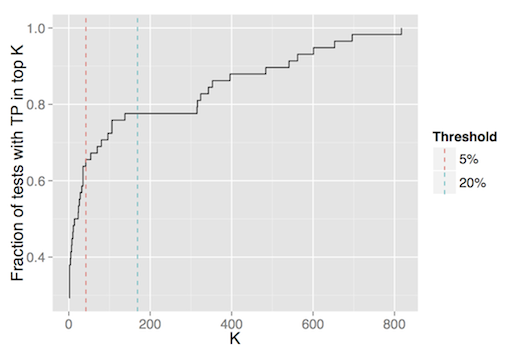
\includegraphics[width=3.5in]{resultcdf.png}
\caption{Cumulative distribution of percentile rank over test examples}
\label{fig_sim}
\end{figure}


\section{Continuing Work}

We believe that by improving our featureset and adding RLSC, we will
be able to further improve our classification accuracy. There are a
number of tasks we hope to work on in order to both increase our
accuracy and to increase our understanding of our results.

\begin{itemize}
\item Adding the regularized least squares classifier.
\item Adding additional features.
\item Studying which features are most predictive, and possibly
  removing those that are not.
\item Studying the effect of aggregating tweets for prediction rather
  than evaluating each tweet's distance individually.
\item Studying the effect of the number of available tweets in a feed
  on prediction accuracy.
\item Continuing to collect data from additional arbitrary streams to
  better understand how the algorithm might perform at larger scales.
\item Add more labeled Twitter account pairs to help smooth the effect
  of odd accounts (both positive and negative) in our test data.
\item Explore methods to determine prediction confidence and applying
thresholds to measure specificity, sensitivity/recall, and precision.
\end{itemize}

\section{Conclusion}

We are encouraged by our initial result. The algorithm exhibits
excellent accuracy in cross validation, and even does fairly well in
the general use case where the test stream comes from a different
Twitter account by the same author. We expected less accuracy from
Twitter than from the blog or email data used in previous work becuase
the amount of data is so much smaller. So the work is promising and
there is a substantial opportunity for continued exploration..

% An example of a floating figure using the graphicx package.
% Note that \label must occur AFTER (or within) \caption.
% For figures, \caption should occur after the \includegraphics.
% Note that IEEEtran v1.7 and later has special internal code that
% is designed to preserve the operation of \label within \caption
% even when the captionsoff option is in effect. However, because
% of issues like this, it may be the safest practice to put all your
% \label just after \caption rather than within \caption{}.
%
% Reminder: the "draftcls" or "draftclsnofoot", not "draft", class
% option should be used if it is desired that the figures are to be
% displayed while in draft mode.
%
%\begin{figure}[!t]
%\centering
%\includegraphics[width=2.5in]{myfigure}
% where an .eps filename suffix will be assumed under latex, 
% and a .pdf suffix will be assumed for pdflatex; or what has been declared
% via \DeclareGraphicsExtensions.
%\caption{Simulation Results}
%\label{fig_sim}
%\end{figure}

% Note that IEEE typically puts floats only at the top, even when this
% results in a large percentage of a column being occupied by floats.


% An example of a double column floating figure using two subfigures.
% (The subfig.sty package must be loaded for this to work.)
% The subfigure \label commands are set within each subfloat command, the
% \label for the overall figure must come after \caption.
% \hfil must be used as a separator to get equal spacing.
% The subfigure.sty package works much the same way, except \subfigure is
% used instead of \subfloat.
%
%\begin{figure*}[!t]
%\centerline{\subfloat[Case I]\includegraphics[width=2.5in]{subfigcase1}%
%\label{fig_first_case}}
%\hfil
%\subfloat[Case II]{\includegraphics[width=2.5in]{subfigcase2}%
%\label{fig_second_case}}}
%\caption{Simulation results}
%\label{fig_sim}
%\end{figure*}
%
% Note that often IEEE papers with subfigures do not employ subfigure
% captions (using the optional argument to \subfloat), but instead will
% reference/describe all of them (a), (b), etc., within the main caption.


% An example of a floating table. Note that, for IEEE style tables, the 
% \caption command should come BEFORE the table. Table text will default to
% \footnotesize as IEEE normally uses this smaller font for tables.
% The \label must come after \caption as always.
%
%\begin{table}[!t]
%% increase table row spacing, adjust to taste
%\renewcommand{\arraystretch}{1.3}
% if using array.sty, it might be a good idea to tweak the value of
% \extrarowheight as needed to properly center the text within the cells
%\caption{An Example of a Table}
%\label{table_example}
%\centering
%% Some packages, such as MDW tools, offer better commands for making tables
%% than the plain LaTeX2e tabular which is used here.
%\begin{tabular}{|c||c|}
%\hline
%One & Two\\
%\hline
%Three & Four\\
%\hline
%\end{tabular}
%\end{table}


% Note that IEEE does not put floats in the very first column - or typically
% anywhere on the first page for that matter. Also, in-text middle ("here")
% positioning is not used. Most IEEE journals/conferences use top floats
% exclusively. Note that, LaTeX2e, unlike IEEE journals/conferences, places
% footnotes above bottom floats. This can be corrected via the \fnbelowfloat
% command of the stfloats package.




% conference papers do not normally have an appendix


% use section* for acknowledgement
% \section*{Acknowledgment}


% The authors would like to thank...
% more thanks here


% trigger a \newpage just before the given reference
% number - used to balance the columns on the last page
% adjust value as needed - may need to be readjusted if
% the document is modified later
%\IEEEtriggeratref{8}
% The "triggered" command can be changed if desired:
%\IEEEtriggercmd{\enlargethispage{-5in}}

% references section

% can use a bibliography generated by BibTeX as a .bbl file
% BibTeX documentation can be easily obtained at:
% http://www.ctan.org/tex-archive/biblio/bibtex/contrib/doc/
% The IEEEtran BibTeX style support page is at:
% http://www.michaelshell.org/tex/ieeetran/bibtex/
%\bibliographystyle{IEEEtran}
% argument is your BibTeX string definitions and bibliography database(s)
%\bibliography{IEEEabrv,../bib/paper}
%
% <OR> manually copy in the resultant .bbl file
% set second argument of \begin to the number of references
% (used to reserve space for the reference number labels box)
\begin{thebibliography}{1}

\bibitem{Abbasi}
Abbasi, Ahmed, and Hsinchun Chen. "Writeprints: A stylometric approach to identity-level identification and similarity detection in cyberspace." ACM Transactions on Information Systems 26.2 (2008): 7.

\bibitem{Narayanan}
Narayanan, Arvind, et al. "On the feasibility of internet-scale author identification." Security and Privacy (SP), 2012 IEEE Symposium on. IEEE, 2012.

\bibitem{Ireland}
Ireland, M.E., \& Pennebaker, J.W. (2010).  Language style matching in writing: Synchrony in essays, correspondence, and poetry.  Journal of Personality and Social Psychology, 99.

\bibitem{Perito}
Perito, Daniele, et al. "How unique and traceable are usernames?." Privacy Enhancing Technologies. Springer Berlin/Heidelberg, 2011.

\end{thebibliography}




% that's all folks
\end{document}


